\documentclass[paper=a4, fontsize=11pt]{article} 

\usepackage[T1]{fontenc} 

\usepackage[utf8]{inputenc}
\usepackage[francais]{babel} 
\usepackage{mathtools}
\usepackage{amssymb}
\usepackage{alltt}
\usepackage{float}
\usepackage{graphicx}
\usepackage[colorinlistoftodos]{todonotes}
\usepackage{geometry}
\usepackage{hyperref}
\usepackage{enumitem}

\usepackage{array,multirow,makecell}
\setcellgapes{1pt}
\makegapedcells
\newcolumntype{R}[1]{>{\raggedleft\arraybackslash }b{#1}}
\newcolumntype{L}[1]{>{\raggedright\arraybackslash }b{#1}}
\newcolumntype{C}[1]{>{\centering\arraybackslash }b{#1}}

\usepackage[hang,small]{caption}

\title{\normalfont \normalsize 
\huge TD 7 : Analyse discriminante linéaire}

\author{Jules Kozolinsky}

\date{}

\begin{document}
\maketitle
\section*{Modèles de régression}
\subsection{}
On représente les données avec la couleur bleu pour la classe $0$ et rouge pour les points de la classe $1$.
\begin{figure}[h]
 \begin{minipage}[b]{.3\linewidth}
 \begin{center}
 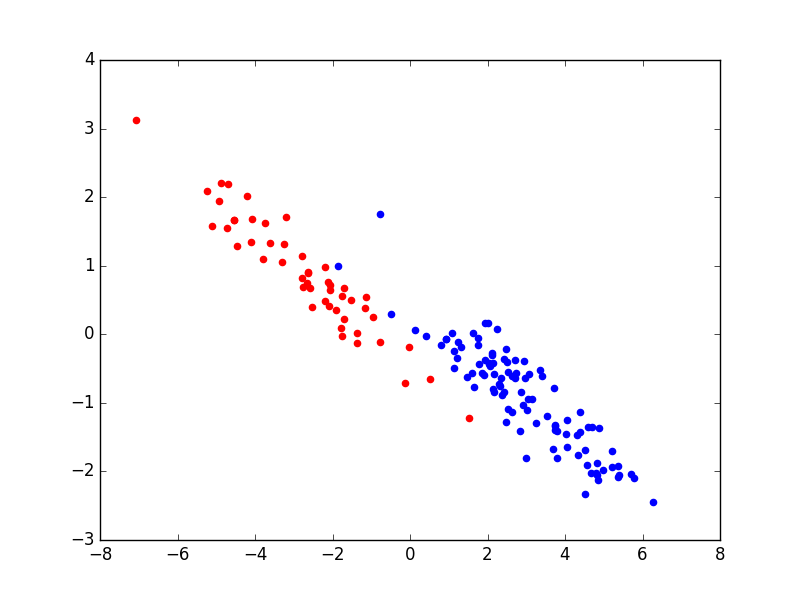
\includegraphics[scale=0.25]{figures/A_train.png}
  \caption*{Ensemble d'apprentissage A}
 \end{center}
 \end{minipage} \hfill
 \begin{minipage}[b]{.3\linewidth}
  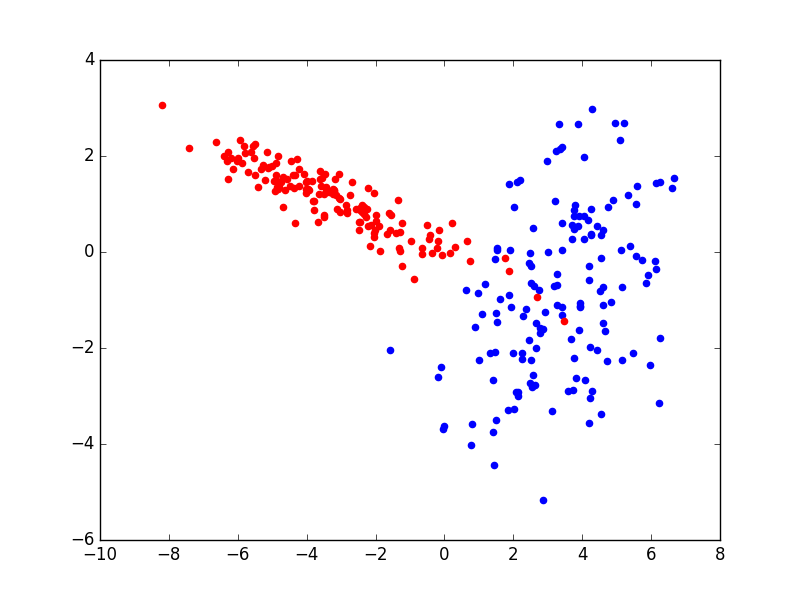
\includegraphics[scale=0.25]{figures/B_train.png}
  \caption*{Ensemble d'apprentissage B}
 \end{minipage} \hfill
 \begin{minipage}[b]{.3\linewidth}
  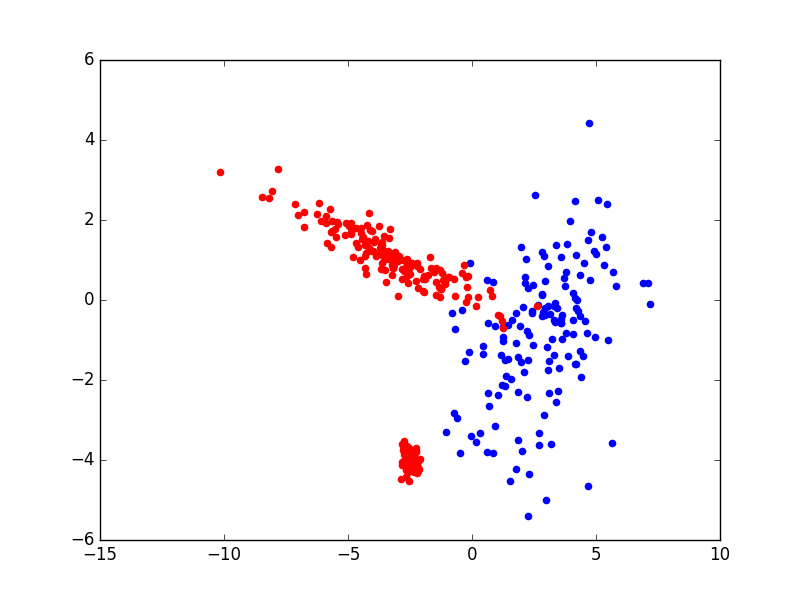
\includegraphics[scale=0.25]{figures/C_train.png}
  \caption*{Ensemble d'apprentissage C}
 \end{minipage}
\end{figure}

On constate que pour les points de l'ensemble d'apprentissage A la covariance semble être la même alors que pour les ensembles d'apprentissage B et C elle semble clairement différente. Enfin, on remarque que la classe $1$ (en rouge) sur l'ensemble d'apprentissage C est bien le mélange de deux Gaussiennes. 

\subsection{}
Pour chaque classe de l'ensemble d'entrainement, on effectue une régression linéaire. Ensuite pour chaque point considéré, on regarde quelle droite est plus proche de notre point et on classifie de la sorte. \\
On obtient les résultats visibles sur la figure ci-dessous (régressions linéaires de la couleur des classes et frontière de classification en noire).\\
\begin{figure}[h]
 \begin{minipage}[b]{.3\linewidth}
 \begin{center}
 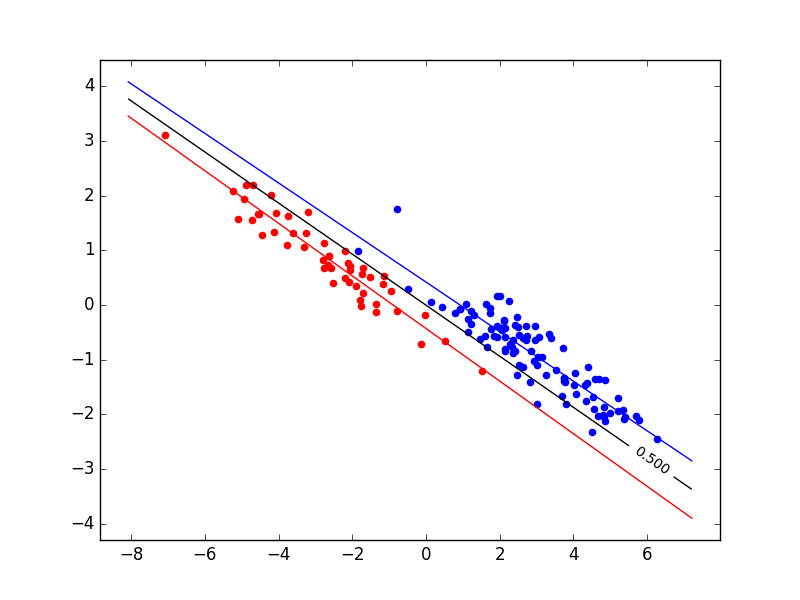
\includegraphics[scale=0.25]{figures/lin_reg_A_train.png}
  \caption*{Ensemble d'apprentissage A \\ (erreur : $6.0\%$)}
 \end{center}
 \end{minipage} \hfill
 \begin{minipage}[b]{.3\linewidth}
  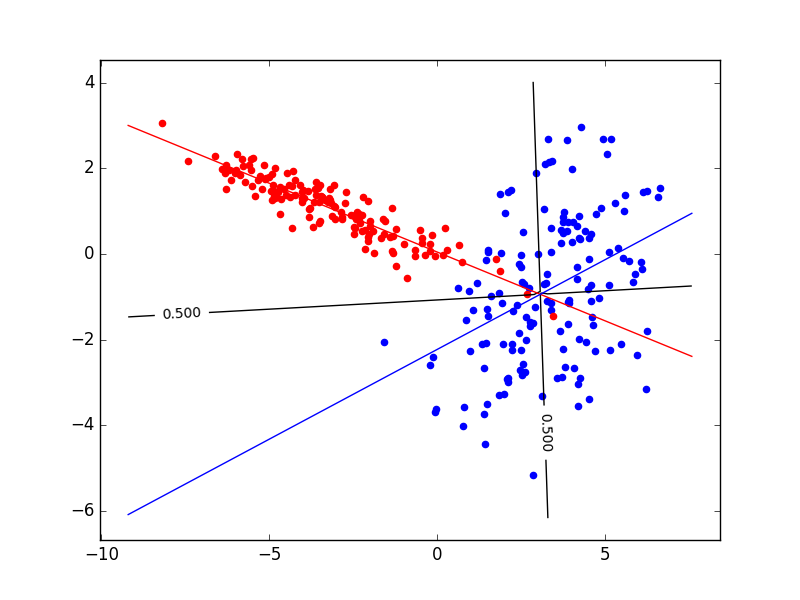
\includegraphics[scale=0.25]{figures/lin_reg_B_train.png}
  \caption*{Ensemble d'apprentissage B \\ (erreur : $16.67\%$)}
 \end{minipage} \hfill
 \begin{minipage}[b]{.3\linewidth}
  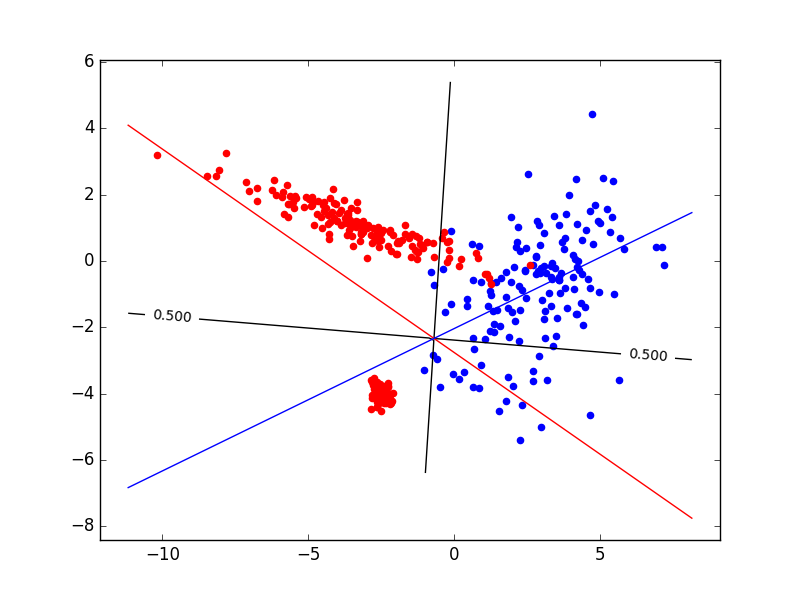
\includegraphics[scale=0.25]{figures/lin_reg_C_train.png}
  \caption*{Ensemble d'apprentissage C \\ (erreur : $35.0\%$)}
 \end{minipage}
\end{figure}
\begin{figure}[h]
 \begin{minipage}[b]{.3\linewidth}
 \begin{center}
 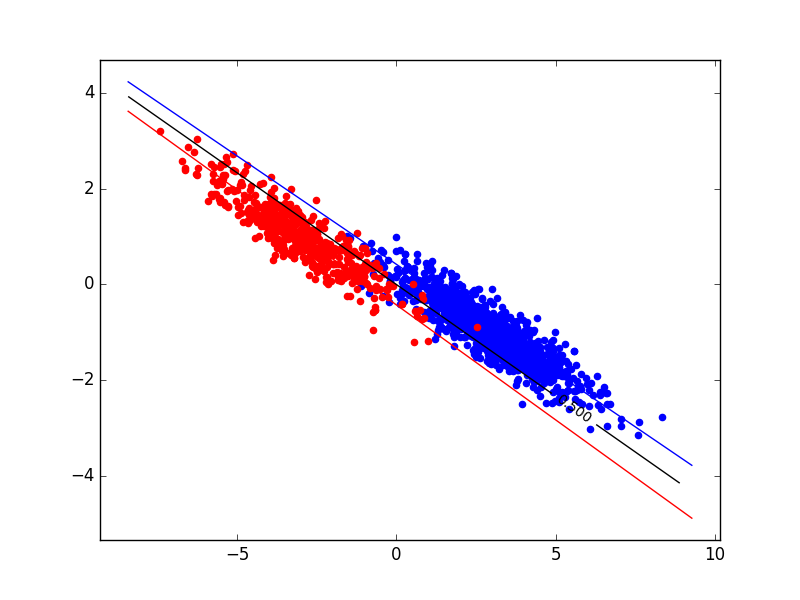
\includegraphics[scale=0.25]{figures/lin_reg_A_test.png}
  \caption*{Ensemble de test A \\ (erreur : $12.34\%$)}
 \end{center}
 \end{minipage} \hfill
 \begin{minipage}[b]{.3\linewidth}
  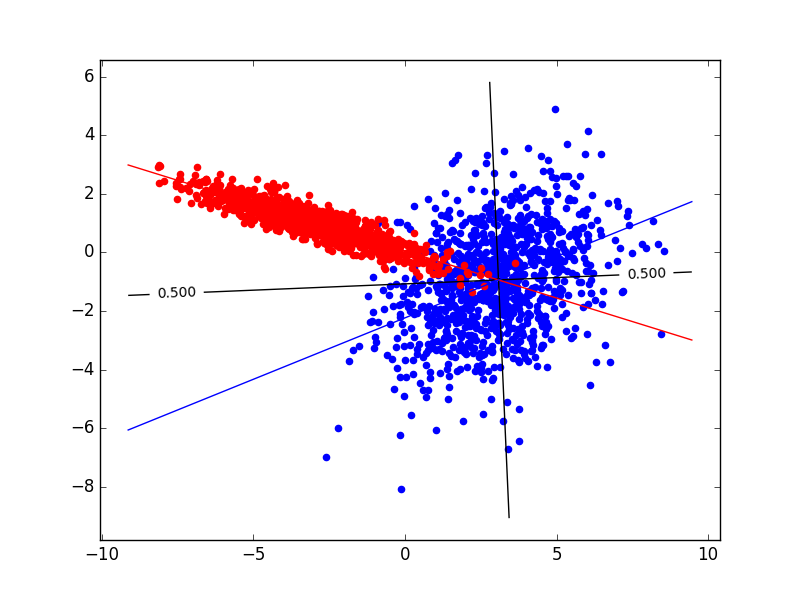
\includegraphics[scale=0.25]{figures/lin_reg_B_test.png}
  \caption*{Ensemble de test B \\ (erreur : $19.45\%$)}
 \end{minipage} \hfill
 \begin{minipage}[b]{.3\linewidth}
  \begin{center}
  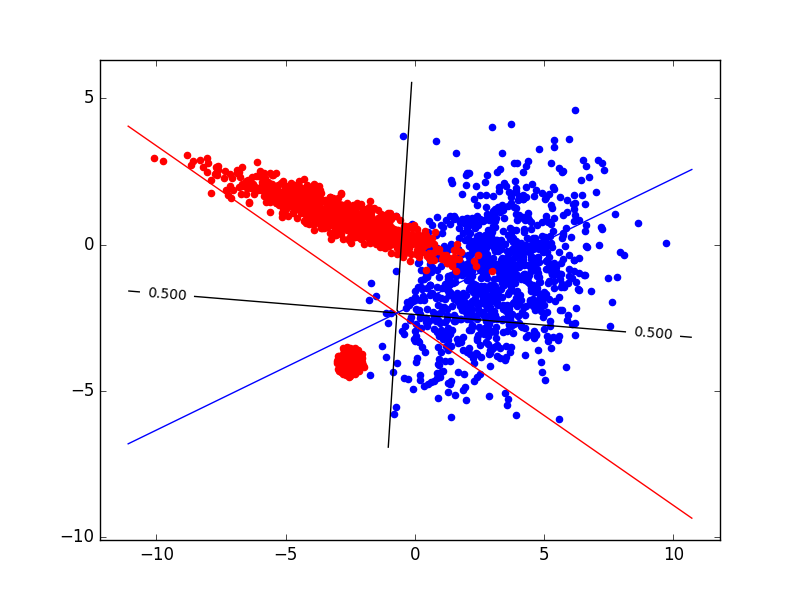
\includegraphics[scale=0.25]{figures/lin_reg_C_test.png}
  \caption*{Ensemble de test C  \\ (erreur : $43.4\%$)}
   \end{center}
 \end{minipage}
\end{figure}
On remarque que quand la covariance est faible alors, les résultats sont plutôt bons (cf données $A$) alors que quand la covariance est de grande, les données sont éparses et la régression linéaire est beaucoup moins précise (cf classe $0$ pour données $B$ et $C$). De plus la classe $1$ des données $C$ est un mélange de deux Gaussiennes, donc les résultats de la régression linéaire pour cette classe sont mauvais. \\
Ainsi, pour de faibles covariance et des distributions gaussiennes simples, la méthode de classification par plug-in de régression linéaire peut s'avérer efficace. 
\subsection{}
Passons à la régression logistique. On maximise la log-vraisemblance, ce qui revient à minimiser l'opposé du risque empirique pour la perte logistique :
\begin{align*}
R_{n}(\omega) = -\frac{1}{n}\sum\limits_{i=1}^{n} y_i\log (\sigma(\omega^{T}x_i)) + (1-y_i)\log(1-\sigma(\omega^{T}x_i))
\end{align*}
Ainsi, en dérivant : 
\begin{align*}
\nabla_{\omega}R_{n}(\omega) = -\frac{1}{n}\sum\limits_{i=1}^{n} x_i(y_i - \sigma(\omega^{T}x_i)) = -\frac{1}{n}X^{T}(y-\mu(\omega)) 
\end{align*}
où $\mu_i(\omega) = \sigma(\omega^{T}x_i)$.\\
On cherche alors à minimiser la fonction $J(\omega) = R_{n}(\omega) + \lambda ||\omega ||^{2}_{2}$

\paragraph{Résolution par méthode de gradient\\}
On effectue une méthode de descente de gradient de pas $\gamma$.
\begin{align*}
\omega_{t+1} = \omega_{t} - \gamma \nabla J(\omega_{t})
\end{align*}

\paragraph{Résultats:\\}
Trois algorithmes d'optimisation ont été implémentés : descente de gradient avec pas constant, avec pas variable (suivant la règle d'Armino) et l'algorithme des moindres carrés pondérés. \\
Pour les données suivantes, on a utilisé l'algorithme des moindres carrés pour la régression logistique avec les données $A$, et la descente de gradient pour les données $B$ et $C$.\\
\begin{figure}[h]
 \begin{minipage}[b]{.3\linewidth}
 \begin{center}
 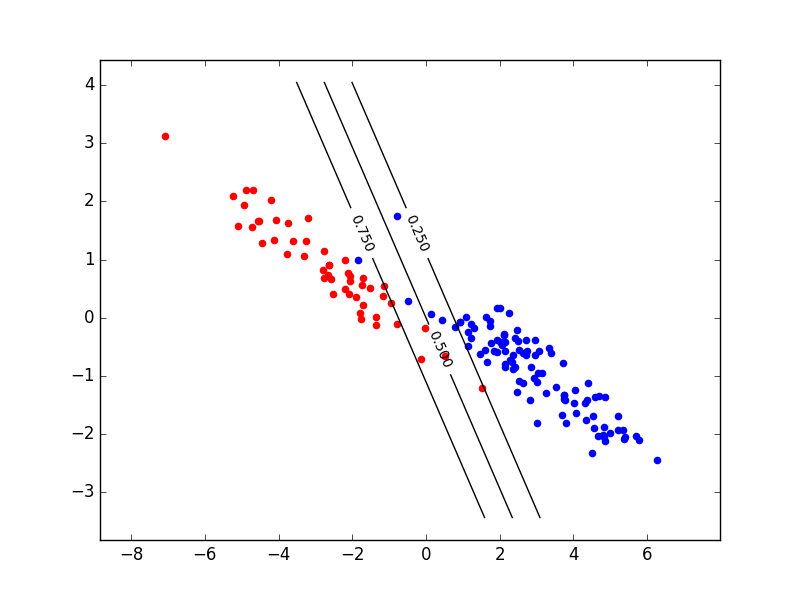
\includegraphics[scale=0.25]{figures/log_reg_A_train.png}
  \caption*{Ensemble d'apprentissage A \\ (erreur : $2.7\%$)}
 \end{center}
 \end{minipage} \hfill
 \begin{minipage}[b]{.3\linewidth}
  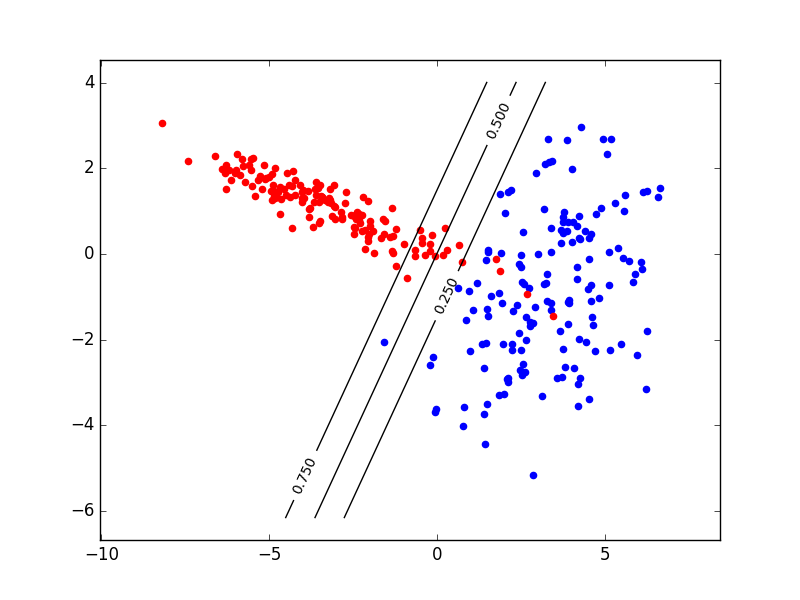
\includegraphics[scale=0.25]{figures/log_reg_B_train.png}
  \caption*{Ensemble d'apprentissage B \\ (erreur : $3.0\%$)}
 \end{minipage} \hfill
 \begin{minipage}[b]{.3\linewidth}
  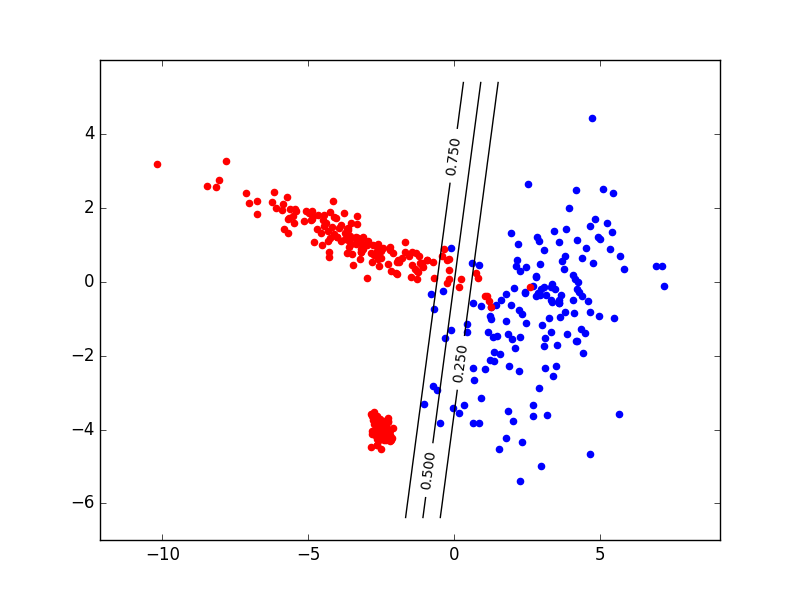
\includegraphics[scale=0.25]{figures/log_reg_C_train.png}
  \caption*{Ensemble d'apprentissage C \\ (erreur : $4.25\%$)}
 \end{minipage}
\end{figure}
\begin{figure}[h]
 \begin{minipage}[b]{.3\linewidth}
 \begin{center}
 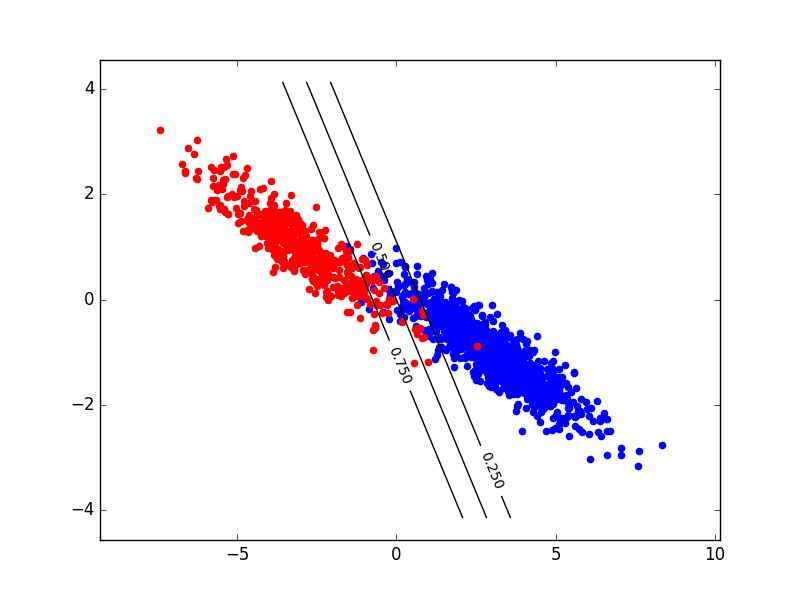
\includegraphics[scale=0.25]{figures/log_reg_A_test.png}
  \caption*{Ensemble de test A \\ (erreur : $2.27\%$)}
 \end{center}
 \end{minipage} \hfill
 \begin{minipage}[b]{.3\linewidth}
  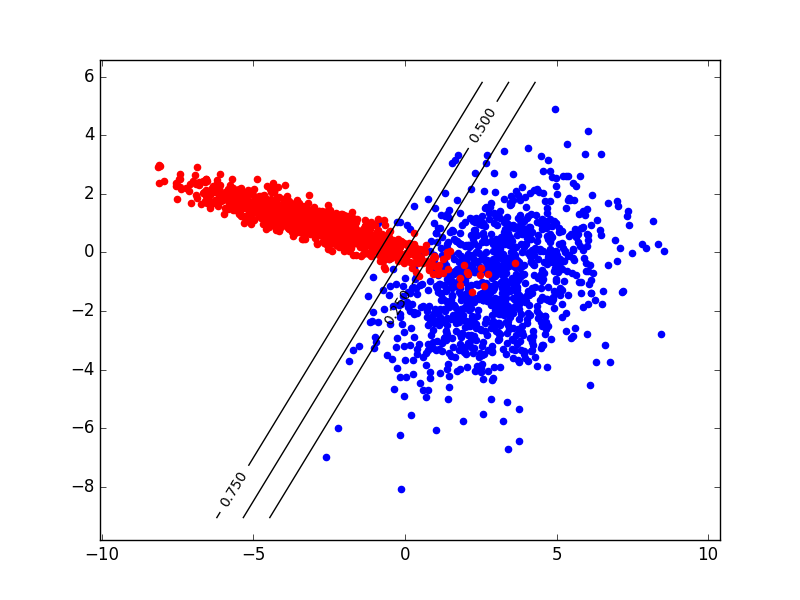
\includegraphics[scale=0.25]{figures/log_reg_B_test.png}
  \caption*{Ensemble de test B \\ (erreur : $4.15\%$)}
 \end{minipage} \hfill
 \begin{minipage}[b]{.3\linewidth}
  \begin{center}
  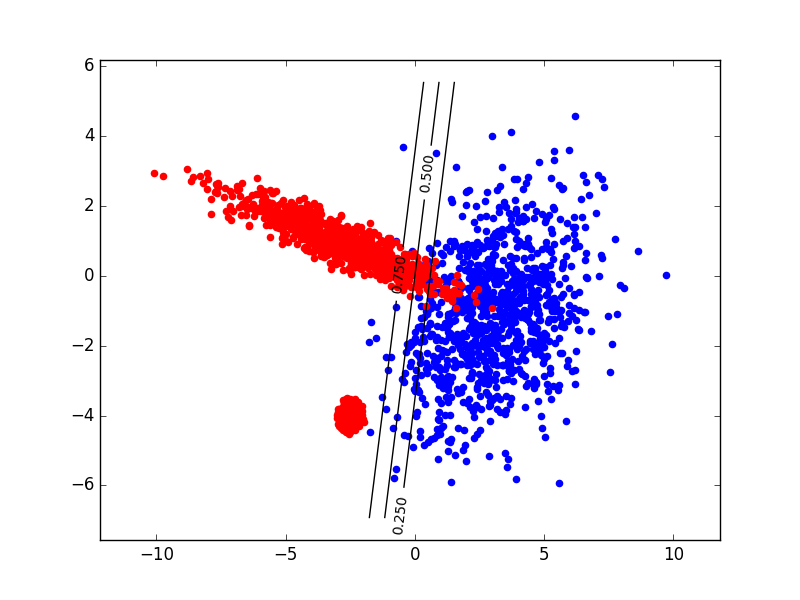
\includegraphics[scale=0.25]{figures/log_reg_C_test.png}
  \caption*{Ensemble de test C  \\ (erreur : $2.77\%$)}
   \end{center}
 \end{minipage}
\end{figure}

Note : ici on représente la frontière de séparation (probabilité $0.5$) ainsi que les lignes de niveau pour $P(Y=1|X=x) = 0.25$ et $P(Y=1|X=x) = 0.75$.
\paragraph{Commentaires:\\}
Les résultats sont bien meilleurs que pour la méthode de classification par plug-in de la régression linéaire. Toutefois on remarque lorsque les données se "mélange", le modèle linéaire de $f$ fait défaut. On pourrait penser aux méthodes à noyaux pour se débarrasser du modèle de $f$.

\section*{Discriminant de Fisher}
On modélise les données par des nuages gaussiens sur $\mathbb{R}^{p}$ de distribution $\mathcal{N}(\mu_0,\Sigma_0)$ et $\mathcal{N}(\mu_1,\Sigma_1)$, respectivement pour les classes 0 et 1. Soit $f_{\mu_0,\Sigma_0}$ et $f_{\mu_1,\Sigma_1}$ les fonctions de densité des nuages gaussiens, tels que :
\begin{align*}
f_{\mu_i,\Sigma_i}=\dfrac{1}{\sqrt{(2\pi)^{p}\det(\Sigma_i)}}e^{-\frac{1}{2}(x-\mu_i)^{T}\Sigma_{i}^{-1}(x-\mu_i)}
\end{align*}
On considèrera seulement dans un second temps que $\Sigma_0 = \Sigma_1 = \Sigma$.
\subsection{a) b)}
Soit $A \in \mathbb{R}^n, i \in \lbrace 0,1 \rbrace$, on a : 
\begin{align*}
P(X \in A \wedge Y = 1) = P(X \in A | Y = 1)P(Y=1) &= \int_{A} f_{\mu_1,\Sigma_1}(x)P(Y=1)d\mu(x) \\
&= \int_{A} \dfrac{f_{\mu_1,\Sigma_1}(x)}{f_{X}(x)}\pi dP(x)
\end{align*}
où $f_X$ est la fonction de densité de la variable aléatoire $X$ :
\begin{align*}
P(X \in A)&=P(Y =0)P(X \in A | Y =0)+P(Y =1)P(X \in A|Y =1) \\
&= (1-\pi)\int_{A} f_{\mu_0,\Sigma_0} + \pi\int_{A} f_{\mu_1,\Sigma_1} 
=  \int_{A} (1-\pi)f_{\mu_0,\Sigma_0} + \pi f_{\mu_1,\Sigma_1}  \\
&= \int_{A} f_{X}
\end{align*}
Ainsi, en définissant la probabilité conditionnelle comme un noyau de transition par rapport à $X$ :
\begin{align*}
P(Y=1|X=x) &= \dfrac{P(Y=1 \wedge X=x)}{P(X=x)} = \dfrac{\pi  f_{\mu_1,\Sigma_1} }{(1-\pi)f_{\mu_0,\Sigma_0} + \pi f_{\mu_1,\Sigma_1} }\\
&= \dfrac{1}{1+\dfrac{(1-\pi)}{\pi}\dfrac{f_{\mu_0,\Sigma_0}}{f_{\mu_1,\Sigma_1}}} \\
&= \sigma(f(x)) 
\end{align*}
où $f(x) = \log(\dfrac{f_{\mu_1,\Sigma_1}}{f_{\mu_0,\Sigma_0}}) + \log(\dfrac{\pi}{1-\pi})$.\\
Le modèle conditionnel de $P(Y|X=x)$ induit par le modèle génératif choisi corresponds donc bien à un modèle probabiliste de classification linéaire de même forme que la régression logistique. 

\subsection*{c)}
On a $\pi = \dfrac{1}{n}\sum\limits_{i=1}^{n} y_i$ et posant $\theta = (\mu_1,\mu_0,\Sigma_1,\Sigma_0) \in (\mathbb{R}^{p},\mathbb{R}^{p},\mathcal{S}_{p}(\mathbb{R}),\mathcal{S}_{p}(\mathbb{R}))$, 
\begin{align*}
f_{\theta}(x) &= \log(\dfrac{f_{\mu_1,\Sigma_1}}{f_{\mu_0,\Sigma_0}}) + \log(\dfrac{\pi}{1-\pi}) \\
&= \log(\dfrac{\dfrac{1}{\sqrt{(2\pi)^{p}\det(\Sigma_1)}}e^{-\frac{1}{2}(x-\mu_1)^{T}\Sigma_{1}^{-1}(x-\mu_1)}}
					{\dfrac{1}{\sqrt{(2\pi)^{p}\det(\Sigma_0)}}e^{-\frac{1}{2}(x-\mu_0)^{T}\Sigma_{0}^{-1}(x-\mu_0)}}) + \log(\dfrac{\pi}{1-\pi}) \\
&= -\frac{1}{2}(x-\mu_1)^{T}\Sigma_{1}^{-1}(x-\mu_1) +  \frac{1}{2}(x-\mu_0)^{T}\Sigma_{0}^{-1}(x-\mu_0) + \dfrac{1}{2}\log(\dfrac{\det(\Sigma_0)}{\det(\Sigma_1)}) + \log(\dfrac{\pi}{1-\pi})
\end{align*}
Ainsi, 
\begin{align*}
\nabla_{\mu_1}f_{\theta}(x) = \Sigma_{1}^{-1}(x-\mu_{1}) \\
\nabla_{\mu_0}f_{\theta}(x) = -\Sigma_{0}^{-1}(x-\mu_{0}) 
\end{align*}
\paragraph{Calcul de $\nabla_{\Sigma_1}f_{\theta}(x)$\\}
1) On pose $\varphi(M) = A^{T}M^{-1}A$ où $M \in \mathcal{M}_{p}(\mathbb{R})$ et $A \in \mathbb{R}^{n}$. \\
Ainsi $\varphi = h \circ g$ où $h(M) = A^{T}MA$ et $g(M) = M^{-1}$.\\
On a : $dh_{M}(H) = A^{T}HA$ et $dg_{M}(H) = -M^{-1}HM^{-1}$ (on factorise par $M$ quand on calcule $g(M+H)$).\\
D'où $d\varphi_{M}(H) = dh_{g(M)}(dg_{M}(H)) = dh_{M^{-1}}(-M^{-1}HM^{-1}) 
= - A^{T}M^{-1}HM^{-1}A $\\
Ainsi, $\nabla_{M}\varphi(M) = -(M^{-1})^{T}AA^{T}(M^{-1})^{T}$.\\


2) On pose $\psi(M) = \log(\det(M))$ où $M \in \mathcal{M}_{p}(\mathbb{R})$\\
On a : $\dfrac{\partial}{\partial M_{ij}}\log\det(M_{ij}) = \dfrac{1}{det(M)}\frac{\partial \det(M)}{\partial M_{ij}}= \dfrac{1}{det(M)} Cof_{ij}(M) = ((M^{-1})^{T})_{ij}$.\\
Ainsi, $\nabla_{M}\psi(M) = (M^{-1})^{T}$.\\


Finalement, 
\begin{align*}
\nabla_{\Sigma_1}f_{\theta}(x) = \dfrac{1}{2}(\Sigma_1^{-1})^{T}(x-\mu_1)(x-\mu_1)^{T}(\Sigma_1^{-1})^{T} - \dfrac{1}{2}(\Sigma_1^{-1})^{T}
\end{align*}
De même, 
\begin{align*}
\nabla_{\Sigma_0}f_{\theta}(x) = -\dfrac{1}{2}(\Sigma_0^{-1})^{T}(x-\mu_0)(x-\mu_0)^{T}(\Sigma_0^{-1})^{T} + \dfrac{1}{2}(\Sigma_0^{-1})^{T}
\end{align*}
Puis, si $\Sigma_0 = \Sigma_1 = \Sigma$, on a : 
\begin{align*}
\nabla_{\Sigma}f_{\theta}(x) = \dfrac{1}{2}(\Sigma^{-1})^{T}((x-\mu_1)(x-\mu_1)^{T}-(x-\mu_0)(x-\mu_0)^{T})(\Sigma^{-1})^{T}
\end{align*}

\paragraph{Principe du maximum de vraisemblance\\}
On souhaite minimiser $-\mathbb{E}(\log(P_{\theta}(Y|X))$, soit, d'après la question $b)$, le risque : 
\begin{align*}
R_n(\theta) &= -\frac{1}{n}\sum\limits_{i=1}^{n} y_i\log (\sigma(f_{\theta}(x_i))) + (1-y_i)\log(1-\sigma(f_{\theta}(x_i)))
\end{align*}
On pose $\varphi(x) =  y\log (\sigma(x)) + (1-y)\log(1-\sigma(x))$ et on a
$\varphi'(x) = y - \sigma(x)$.\\
Ainsi, 
\begin{align*}
\nabla_{\mu_1}R_n(\theta) &= -\dfrac{1}{n}\sum\limits_{i=1}^{n} \nabla_{\mu_1}f_{\theta}(x_i)(y_i - \sigma(f_{\theta}(x_i))) \\
&= -\dfrac{1}{n}\sum\limits_{i=1}^{n} \Sigma_{1}^{-1}(x_i-\mu_{1})(y_i - \sigma(f_{\theta}(x_i))) \\
&= -\dfrac{1}{n}\Sigma_{1}^{-1} X_{\mu_1}^{T}Y_{\nu}
\end{align*}
où $\nu_i(\theta) = \sigma(f_{\theta}(x_i))$.\\
De même, 
\begin{align*}
\nabla_{\mu_0}R_n(\theta) =  \dfrac{1}{n}\Sigma_{0}^{-1} X_{\mu_1}^{T}Y_{\nu}
\end{align*}
Puis, 
\begin{align*}
\nabla_{\Sigma_1}R_n(\theta) &= -\dfrac{1}{n}\sum\limits_{i=1}^{n} \nabla_{\Sigma_1}f_{\theta}(x_i)(y_i - \sigma(f_{\theta}(x_i))) \\
&= -\dfrac{1}{2n}(\Sigma_1^{-1})^{T}\sum\limits_{i=1}^{n} ((x_i-\mu_1)(x_i-\mu_1)^{T}(\Sigma_1^{-1})^{T} - I)(y_i - \sigma(f_{\theta}(x_i))) \\
\nabla_{\Sigma_0}R_n(\theta) &= -\dfrac{1}{n}\sum\limits_{i=1}^{n} \nabla_{\Sigma_0}f_{\theta}(x_i)(y_i - \sigma(f_{\theta}(x_i))) \\
&= \dfrac{1}{2n}(\Sigma_0^{-1})^{T}\sum\limits_{i=1}^{n} ((x_i-\mu_0)(x_i-\mu_0)^{T}(\Sigma_0^{-1})^{T} - I)(y_i - \sigma(f_{\theta}(x_i)))
\end{align*}
Et 
\begin{align*}
\nabla_{\Sigma}R_n(\theta) &= -\dfrac{1}{n}\sum\limits_{i=1}^{n} \nabla_{\Sigma}f_{\theta}(x_i)(y_i - \sigma(f_{\theta}(x_i))) \\
&= \dfrac{1}{2n}(\Sigma^{-1})^{T}\sum\limits_{i=1}^{n}((x-\mu_0)(x-\mu_0)^{T}-(x-\mu_1)(x-\mu_1)^{T})(\Sigma^{-1})^{T}(y_i - \sigma(f_{\theta}(x_i)))
\end{align*}

\paragraph{Aparté : Pourquoi ne pas apprendre $\Sigma_i^{-1}$?\\}
Remarquons que $f_{\theta}$ ne dépend que de l'inverse de $\Sigma_i$, on pourrait donc être tenté d'apprendre directement $\Sigma_i^{-1}$ et non $\Sigma_i$ (car $\forall M\in \mathcal{M}_{p}(\mathbb{R}), \det(M^{-1}) = \dfrac{1}{\det(M)}$).\\
On note $\alpha = (\mu_1,\mu_0,\Sigma_1^{-1},\Sigma_0^{-1}) =  (\mu_1,\mu_0,\Omega_1,\Omega_0)\in (\mathbb{R}^{p},\mathbb{R}^{p},\mathcal{M}_{p}(\mathbb{R}),\mathcal{M}_{p}(\mathbb{R}))$ (on perds peut-être la symétrie).\\
Donc : 
\begin{align*}
&f_{\alpha}(x) = -\frac{1}{2}(x-\mu_1)^{T}\Omega_1(x-\mu_1) +  \frac{1}{2}(x-\mu_0)^{T}\Omega_0(x-\mu_0) + \dfrac{1}{2}\log(\dfrac{\det(\Omega_1)}{\det(\Omega_0)}) + \log(\dfrac{\pi}{1-\pi})\\
&\nabla_{\mu_1}f_{\alpha}(x) = \Omega_{1}(x-\mu_{1}) \\
&\nabla_{\mu_0}f_{\alpha}(x) = -\Omega_{0}(x-\mu_{0}) \\
&\nabla_{\Omega_1}f_{\alpha}(x) = -\dfrac{1}{2}(x-\mu_{1})(x-\mu_{1})^{T} +\dfrac{1}{2}(\Omega_1^{-1})^{T}\\
&\nabla_{\Omega_0}f_{\alpha}(x) = \dfrac{1}{2}(x-\mu_{0})(x-\mu_{0})^{T} - \dfrac{1}{2}(\Omega_0^{-1})^{T}\\
\end{align*}
Et 
\begin{align*}
&R_n(\alpha) = -\frac{1}{n}\sum\limits_{i=1}^{n} y_i\log (\sigma(f_{\alpha}(x_i))) + (1-y_i)\log(1-\sigma(f_{\alpha}(x_i)))\\
&\nabla_{\mu_1}R_n(\alpha) = -\dfrac{1}{n}\Omega_{1} X_{\mu_1}^{T}Y_{\nu}\\
&\nabla_{\mu_0}R_n(\alpha) =  \dfrac{1}{n}\Omega_{0} X_{\mu_1}^{T}Y_{\nu}\\
&\nabla_{\Omega_1}R_n(\theta) = \dfrac{1}{2n}\sum\limits_{i=1}^{n}   ((x-\mu_{1})(x-\mu_{1})^{T} -(\Omega_1^{-1})^{T}) (y_i - \sigma(f_{\theta}(x_i))) \\
&\nabla_{\Omega_0}R_n(\theta) = -\dfrac{1}{2n}\sum\limits_{i=1}^{n}   ((x-\mu_{0})(x-\mu_{0})^{T} -(\Omega_0^{-1})^{T}) (y_i - \sigma(f_{\theta}(x_i))) \\
&\nabla_{\Omega}R_n(\theta) = \dfrac{1}{2n}\sum\limits_{i=1}^{n}   ((x-\mu_{1})(x-\mu_{1})^{T}-(x-\mu_{0})(x-\mu_{0})^{T} ) (y_i - \sigma(f_{\theta}(x_i))) 
\end{align*}
On remarque que dans l'hypothèse $\Sigma_1 = \Sigma_0$ que l'ont fait pour la méthode LDA, l'inverse de $\Omega$ n'apparaît pas. On n'a à calculer aucune inverse de matrice. Cela pourrait permettre de gagner du temps de calcul.
\paragraph{Résultats :}cf Annexe
\subsection*{d)}
\paragraph{Résultats:} cf Annexe
\paragraph{Commentaires :\\} Comme le nom de l'algorithme l'indique, les frontières de séparation ne sont plus linéaire, mais quadratique. On s'est en effet donné un degré de liberté en plus. 

\subsection{} Plutôt que de représenter les quatre classifieurs sur le même schéma, j'ai choisi d'afficher les résultats pour chaque question. 

\subsection{Tableau des taux d'erreurs de classifications} 
\begin{center}
\begin{tabular}{|L{3.5cm}||C{1.5cm}|C{1.5cm}||C{1.5cm}|C{1cm}||C{1.5cm}|C{1.5cm}|}
\hline  & $A\_$train &  $A\_$test &  $B\_$train & $B\_$test & $C\_$train & $C\_$test\\
\hline  Régression linéaire & $6 \%$ & $12.34\%$ & $16.67\%$ & $19.45\%$ & $35\%$ & $43.4\%$  \\
\hline  Régression logistique & $2.7 \%$ & $2.27\%$ & $3\%$ & $4.15\%$ & $4.25\%$ & $2.77\%$ 
\\
\hline  LDA & $2.67 \%$ & $2\%$ & $2\%$ & $4.75\%$ & $4\%$ & $2.23\%$ 
\\
\hline  QDA & $1.34 \%$ & $2.07\%$ & $1.76\%$ & $2.20\%$ & $1.25\%$ & $1.93\%$  \\
\hline
\end{tabular}
\end{center}

\subsection{Commentaires} 
La méthode QDA est très efficace sur l'ensemble des données là où les méthodes linéaires (LDA et régression logistique) sont meilleures sur les données de faibles covariance et de Gaussiennes simples. On remarque une très faible différence entre LDA et la régression logistique, compréhensible d'après la question $4b)$ (le modèle de $f$ ne semble pas importer tant que ça pour ces exemples). La première méthode par plug-in est inefficace. 

\subsection{Méthode des $k$-plus proches voisins}
Pour la méthode des $k$ plus proches voisins, on ajuste $k$ par validation croisée. On choisit donc aléatoirement des indices puis on découpe notre intervalle pour lancer localement un $k-PPV$. C'est pourquoi lors de chaque exécution de l'algorithme, on peut avoir un $k$ optimum différent. \\Ici un tableau récapitulatif avec des $k$ possibles (en pratique les plus souvent donnés par l'algorithme de validation croisée). \\
\begin{center}
\begin{tabular}{|R{2cm}||C{1.5cm}|C{1.5cm}||C{1.5cm}|C{1cm}||C{1.5cm}|C{1.5cm}|}
\hline  & $A\_$train &  $A\_$test &  $B\_$train & $B\_$test & $C\_$train & $C\_$test\\
\hline  $k=1$ & $0 \%$ & $2.47\%$ & $0\%$ & $4.0\%$ & $0\%$ & $2.3\%$  \\
\hline  $k=2$ & $2 \%$ & $2.67\%$ & $1\%$ & $2.85\%$ & $0.5\%$ & $2.13\%$ 
\\
\hline  $k=3$ & $3.33 \%$ & $2.06\%$ & $1\%$ & $3.25\%$ & $3.5\%$ & $2.1\%$  \\
\hline
\end{tabular}
\end{center}
La méthodes des $k$ plus proches voisins est remarquablement efficace étant donné qu'elle ne considère pas de modèle pour $f$. Elle l'est d'autant plus que le modèle des fonctions se complexifient (comme sur les données $C$). Cette efficacité du taux d'erreur est compensé par un temps de calcul plus important que les autres méthodes. 

\subsection{}
On considère les données MNIST. On en sélectionne aléatoirement $D=6000$ qu'on partitionne selon $x=\dfrac{1}{3}$, i.e. un tiers de données d'entrainement, deux tiers de données de test. 
\subsubsection*{LDA et QDA à $K$ classes}
Soit $K$ le nombre de classe de notre problème. \\
\paragraph{Modèle \\}
On modélise les données de chaque classe comme un nuage Gaussien de distribution $\mathcal{N}(\mu_k,\Sigma_k)$ pour chaque classe $k$. \\
On note $\forall k \in \lbrace 0,K-1 \rbrace$,
\begin{align*}
f^{k}(x) \doteq f_{\mu_k,\Sigma_k}(x) =\dfrac{1}{\sqrt{(2\pi)^{p}\det(\Sigma_k)}}e^{-\frac{1}{2}(x-\mu_k)^{T}\Sigma_{k}^{-1}(x-\mu_k)}
\end{align*}
Alors : 
\begin{align*}
\nabla_{\mu_k}f^{k}(x) = \Sigma_{k}^{-1}(x-\mu_k)f^{k}(x)
\end{align*}
Et 
\begin{align*}
\nabla_{\Sigma_k}f^{k}(x) = f^{k}(x)(\dfrac{1}{2}(\Sigma_k^{-1})^{T}(x-\mu_k)(x-\mu_k)^{T}(\Sigma_k^{-1})^{T} - \dfrac{1}{2}(\Sigma_k^{-1})^{T}))
\end{align*}
\paragraph{Maximisation de la vraisemblance}
On a, notant $\pi_j = P(Y=j)$ et $h_k = \pi_k f^{k}$, 
\begin{align*}
P(Y=k|X=x) = \dfrac{P(Y=k \wedge X=x)}{P(X=x)} = \dfrac{\pi_k  f_{\mu_k,\Sigma_k} }{\sum\limits_{j=0}^{K-1}\pi_j f_{\mu_j,\Sigma_j}} = 
\dfrac{h_k}{\sum\limits_{j=0}^{K-1} h_j}\\
\end{align*}
On souhaite maximiser la $\log$-vraisemblance. On note le risque :
\begin{align*}
R_n(\theta) &= -\frac{1}{n}\sum\limits_{i=1}^{n} \log(\dfrac{h_{y_i}(x_i)}{\sum\limits_{j=0}^{K-1} h_j(x_i)}) =  -\frac{1}{n}\sum\limits_{i=1}^{n} (\log(h_{y_i}(x_i)) - \log(\sum\limits_{j=0}^{K-1} h_j(x_i)))\\
\end{align*}
On pose alors $\varphi_k(x) = \log(h_k(x)) - \log(\sum\limits_{j=0}^{K-1} h_j(x))$\\
D'où 
\begin{align*}
\nabla_{\mu_k}\varphi_i(x) = \delta_{ik}\dfrac{\nabla_{\mu_k}f^{k}(x)}{f^{k}(x)} - \pi_k\dfrac{\nabla_{\mu_k}f^{k}(x)}{\sum\limits_{j=0}^{K-1} h_j(x)}
\end{align*}
Ainsi, 
\begin{align*}
\nabla_{\mu_k}R_n(\theta) &= -\frac{1}{n}\sum\limits_{i=1}^{n} (\delta_{y_{i}k}\dfrac{\nabla_{\mu_k}f^{k}(x_i)}{f^{k}(x_i)} - \pi_k\dfrac{\nabla_{\mu_k}f^{k}(x_i)}{\sum\limits_{j=0}^{K-1} \pi_j f^{j}(x_i)}) \\
&= -\frac{1}{n}\sum\limits_{i=1}^{n}(\delta_{y_{i}k}\Sigma_{k}^{-1}(x_i-\mu_k) - \Sigma_{k}^{-1}(x-\mu_k)\dfrac{\pi_kf^{k}(x_i)}{\sum\limits_{j=0}^{K-1} \pi_j f^{j}(x_i)})
\end{align*}
De même :
\begin{align*}
\nabla_{\Sigma_k}R_n(\theta) &= -\frac{1}{n}\sum\limits_{i=1}^{n} (\delta_{y_{i}k}\dfrac{\nabla_{\Sigma_k}f^{k}(x_i)}{f^{k}(x_i)} - \pi_k\dfrac{\nabla_{\Sigma_k}f^{k}(x_i)}{\sum\limits_{j=0}^{K-1} \pi_j f^{j}(x_i)}) \\
&=-\frac{1}{2n}\sum\limits_{i=1}^{n}(\delta_{y_ik}(\Sigma_k^{-1})^{T}(x_i-\mu_k)(x_i-\mu_k)^{T}(\Sigma_k^{-1})^{T} - (\Sigma_k^{-1})^{T})) \\&- ((\Sigma_k^{-1})^{T}(x_i-\mu_k)(x_i-\mu_k)^{T}(\Sigma_k^{-1})^{T} - (\Sigma_k^{-1})^{T}))\dfrac{\pi_kf^{k}(x_i)}{\sum\limits_{j=0}^{K-1} \pi_j f^{j}(x_i)})
\end{align*}
\paragraph{Résume\\}
On note : 
\begin{align*}
H_k(x) &= \dfrac{\pi_kf^{k}(x)}{\sum\limits_{j=0}^{K-1} \pi_j f^{j}(x)}\\
A_k(x) &= \Sigma_{k}^{-1}(x-\mu_k)\\
B_k(x) &= (\Sigma_k^{-1})^{T}(x-\mu_k)(x-\mu_k)^{T}(\Sigma_k^{-1})^{T} - (\Sigma_k^{-1})^{T}
\end{align*}
On a finalement : 
\begin{align*}
R_n(\theta) &= -\frac{1}{n}\sum\limits_{i=1}^{n} \log(H_{y_i}(x_i))\\
\nabla_{\mu_k}R_n(\theta) &= \frac{1}{n}\sum\limits_{i=1}^{n}A_k(x_i)(H_k(x_i)-\delta_{y_ik})\\
\nabla_{\Sigma_k}R_n(\theta) &= \frac{1}{2n}\sum\limits_{i=1}^{n}B_k(x_i)(H_k(x_i)-\delta_{y_ik})\\
\end{align*}

\paragraph{Résultats}
Cette méthode est implémentée (pour QDA) et tourne bien, mais elle est très longue à s'exécuter. En effet, des matrices de taille $784,784$ à inverse, 10 classes, même en prenant une centaine de données d'entrainement, le tout est très lent. Ça fonctionne mais je n'ai malheureusement pas de tableaux avec des résultats concluants.\\
Ci-dessous les résultats (rapides) des $k$ plus proches voisins.
\begin{center}
\begin{tabular}{|R{2cm}||C{1.5cm}|C{1.5cm}|}
\hline  & train &  test \\
\hline  $k=1$ & $0\%$ & $9.55\%$ \\
\hline  $k=2$ & $5.4\%$ & $10.3\%$ \\
\hline  $k=3$ & $4.7\%$ & $8.75\%$  \\
\hline  $k=4$ & $5.3\%$ & $9.775\%$  \\
\hline  $k=5$ & $6.5\%$ & $9.225\%$ \\
\hline  $k=6$ & $7.15\%$ & $9.225\%$ \\
\hline
\end{tabular}
\end{center}

\newpage
\section*{Annexe}
\subsection*{LDA}
\begin{figure}[h]
 \begin{minipage}[b]{.3\linewidth}
 \begin{center}
 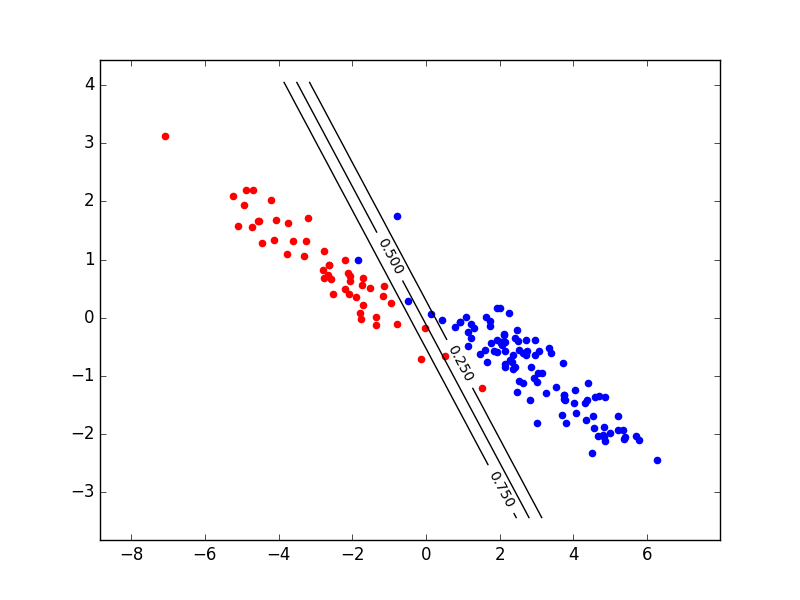
\includegraphics[scale=0.25]{figures/LDA_A_train.png}
  \caption*{Ensemble d'apprentissage A \\ (erreur : $2.67\%$)}
 \end{center}
 \end{minipage} \hfill
 \begin{minipage}[b]{.3\linewidth}
  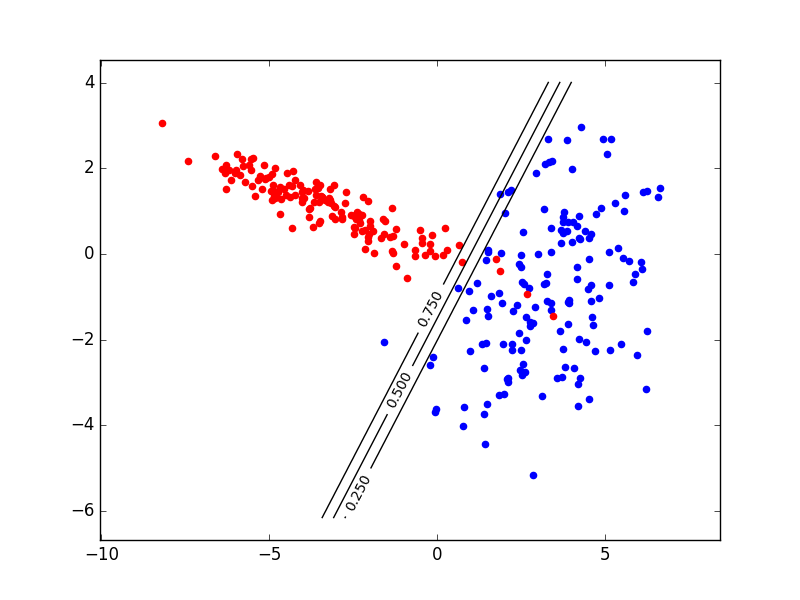
\includegraphics[scale=0.25]{figures/LDA_B_train.png}
  \caption*{Ensemble d'apprentissage B \\ (erreur : $2.0\%$)}
 \end{minipage} \hfill
 \begin{minipage}[b]{.3\linewidth}
  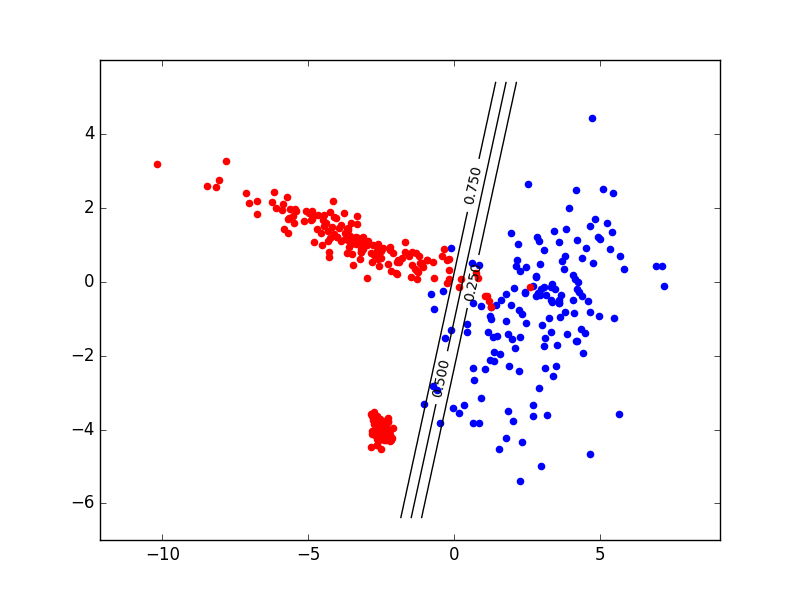
\includegraphics[scale=0.25]{figures/LDA_C_train.png}
  \caption*{Ensemble d'apprentissage C \\ (erreur : $4.0\%$)}
 \end{minipage}
\end{figure}
\begin{figure}[h]
 \begin{minipage}[b]{.3\linewidth}
 \begin{center}
 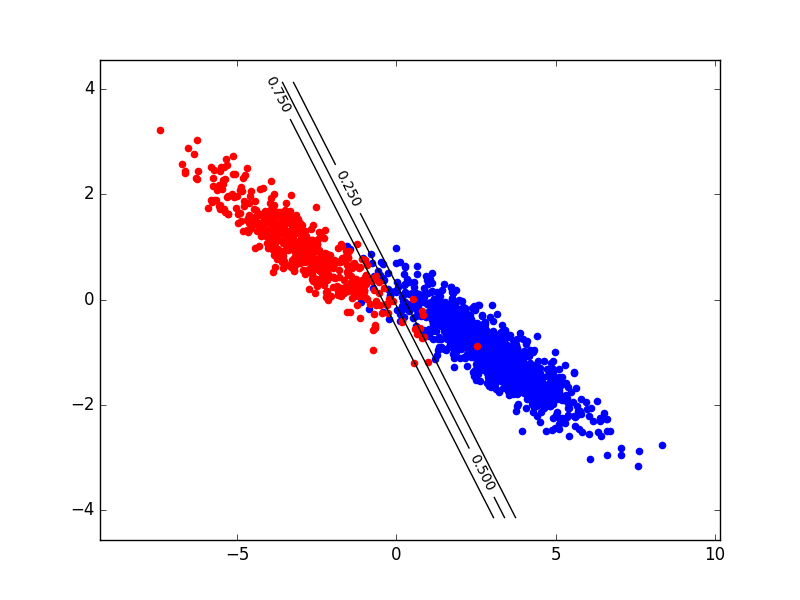
\includegraphics[scale=0.25]{figures/LDA_A_test.png}
  \caption*{Ensemble de test A \\ (erreur : $2.0\%$)}
 \end{center}
 \end{minipage} \hfill
 \begin{minipage}[b]{.3\linewidth}
  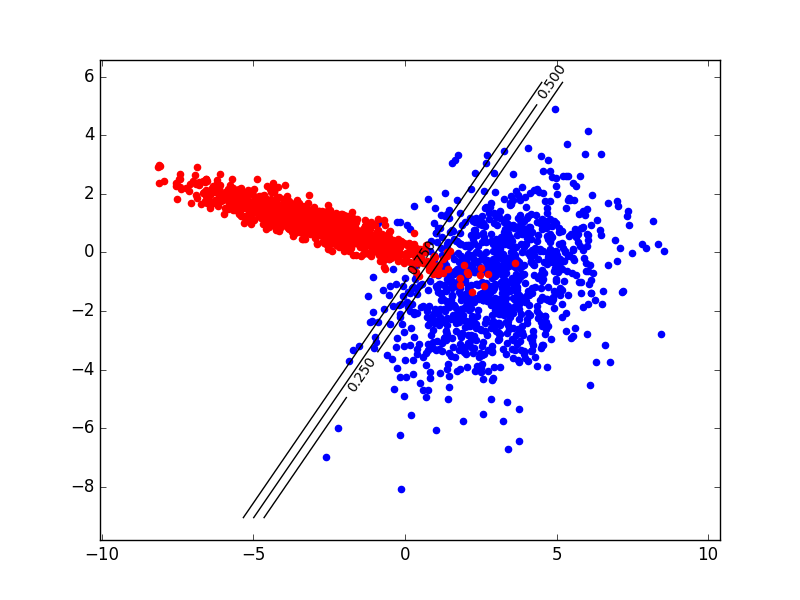
\includegraphics[scale=0.25]{figures/LDA_B_test.png}
  \caption*{Ensemble de test B \\ (erreur : $4.75\%$)}
 \end{minipage} \hfill
 \begin{minipage}[b]{.3\linewidth}
  \begin{center}
  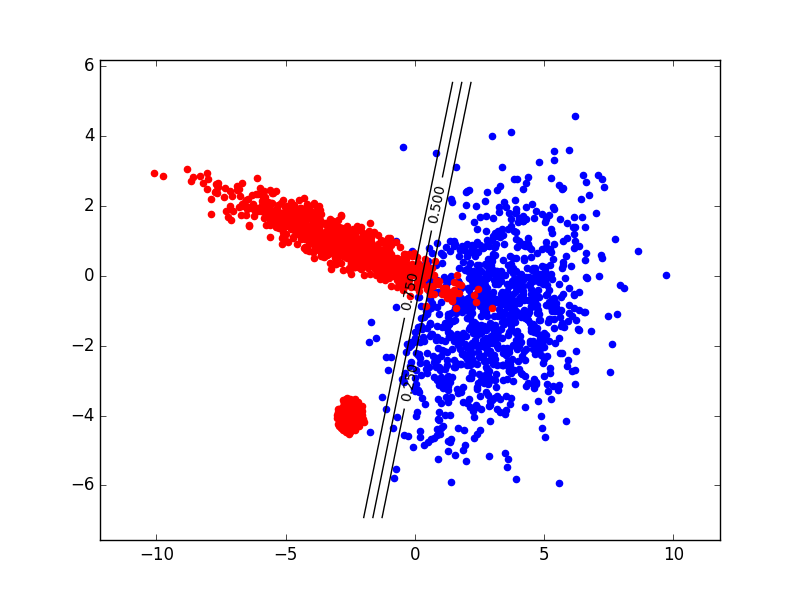
\includegraphics[scale=0.25]{figures/LDA_C_test.png}
  \caption*{Ensemble de test C  \\ (erreur : $2.23\%$)}
   \end{center}
 \end{minipage}
\end{figure}
\newpage
\subsection*{QDA}
\begin{figure}[h]
 \begin{minipage}[b]{.3\linewidth}
 \begin{center}
 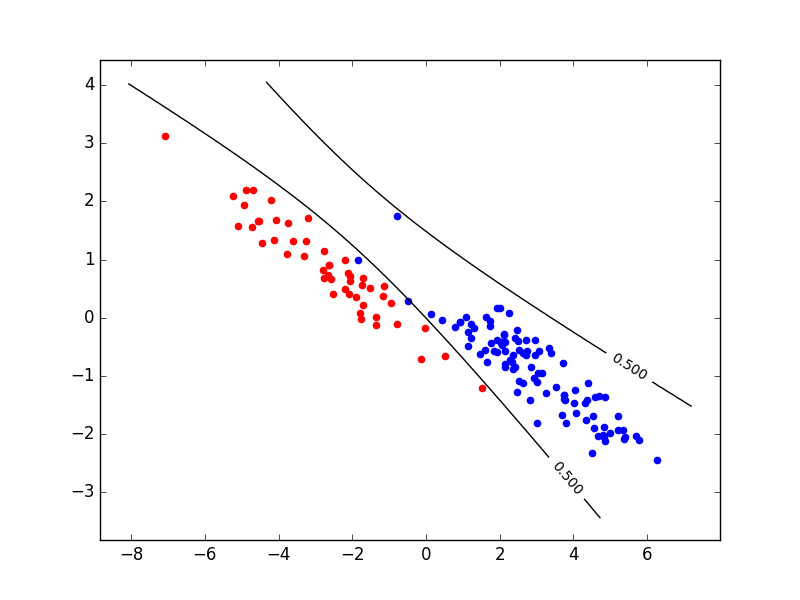
\includegraphics[scale=0.25]{figures/QDA_A_train.png}
  \caption*{Ensemble d'apprentissage A \\ (erreur : $1.34\%$)}
 \end{center}
 \end{minipage} \hfill
 \begin{minipage}[b]{.3\linewidth}
  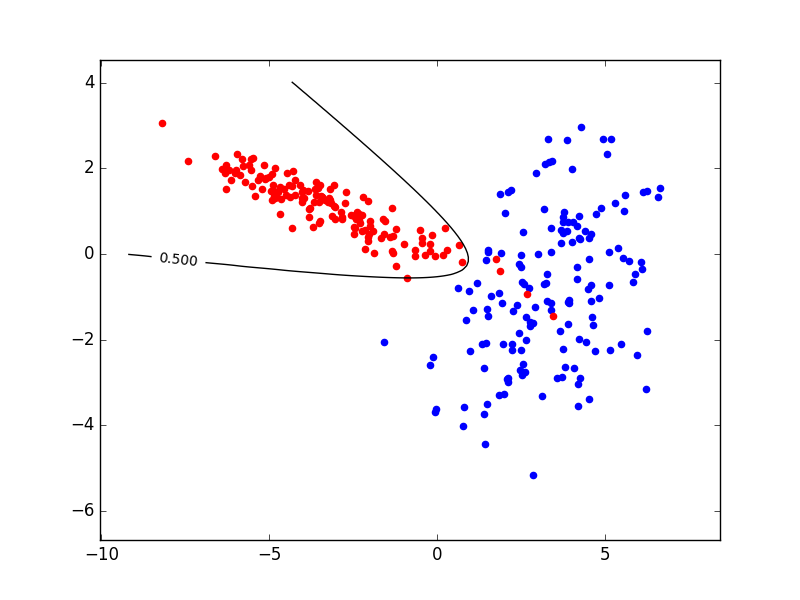
\includegraphics[scale=0.25]{figures/QDA_B_train.png}
  \caption*{Ensemble d'apprentissage B \\ (erreur : $1.67\%$)}
 \end{minipage} \hfill
 \begin{minipage}[b]{.3\linewidth}
  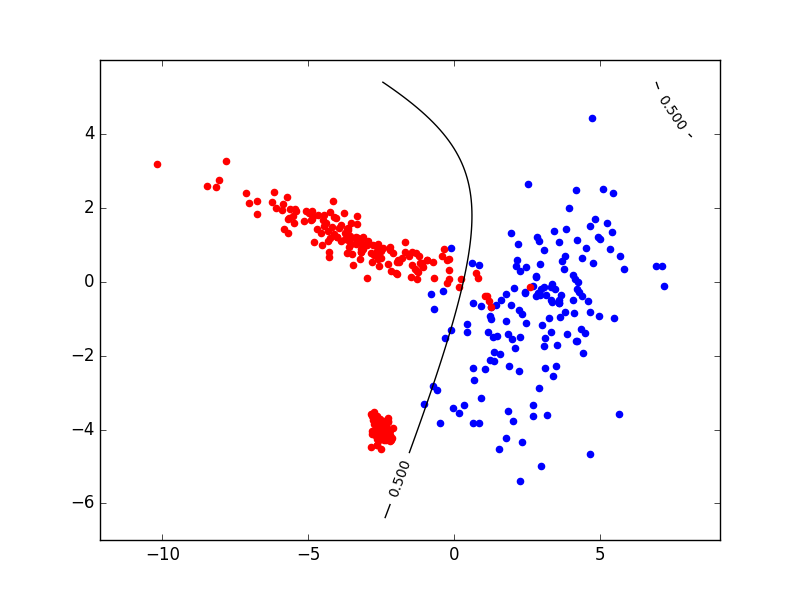
\includegraphics[scale=0.25]{figures/QDA_C_train.png}
  \caption*{Ensemble d'apprentissage C \\ (erreur : $3.5\%$)}
 \end{minipage}
\end{figure}
\begin{figure}[h]
 \begin{minipage}[b]{.3\linewidth}
 \begin{center}
 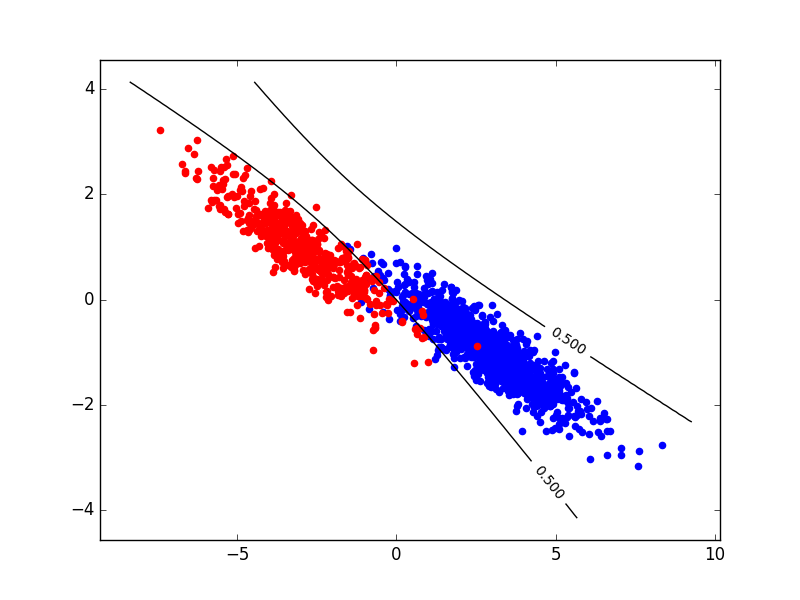
\includegraphics[scale=0.25]{figures/QDA_A_test.png}
  \caption*{Ensemble de test A \\ (erreur : $2.07\%$)}
 \end{center}
 \end{minipage} \hfill
 \begin{minipage}[b]{.3\linewidth}
  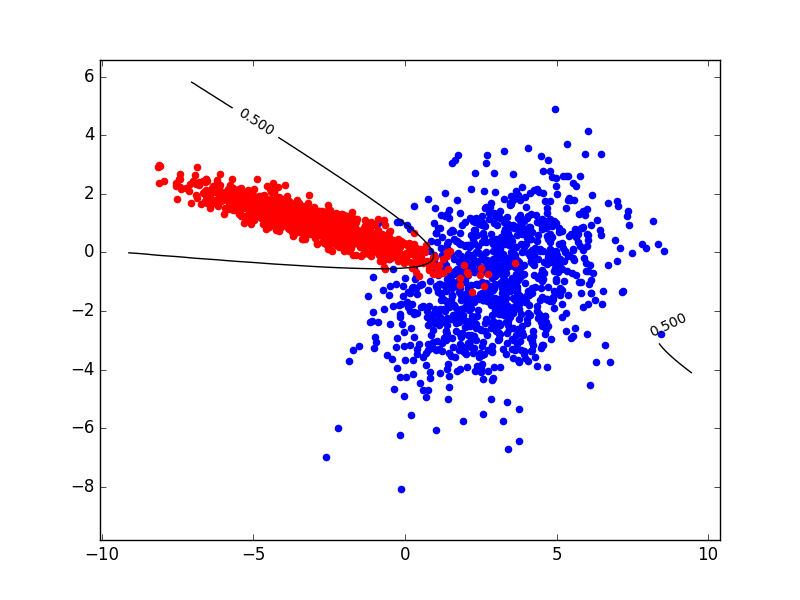
\includegraphics[scale=0.25]{figures/QDA_B_test.png}
  \caption*{Ensemble de test B \\ (erreur : $2.20\%$)}
 \end{minipage} \hfill
 \begin{minipage}[b]{.3\linewidth}
  \begin{center}
  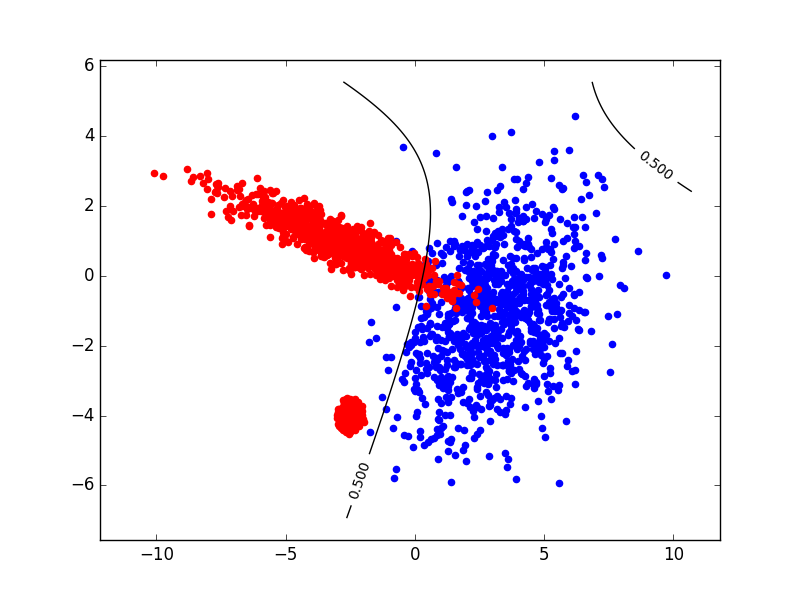
\includegraphics[scale=0.25]{figures/QDA_C_test.png}
  \caption*{Ensemble de test C  \\ (erreur : $2.1\%$)}
   \end{center}
 \end{minipage}
\end{figure}


\end{document}